\documentclass{standalone}
\usepackage{standalone}

\begin{document}

\chapter{Methodology}
This chapter describes our process to detect license plate given an input image, and separation of the individual numbers and character sequence from detected license plate. The input image may come from variety of sources. We have put on a validation method to detect if there is actually a license plate in the input image.


\documentclass{standalone}
\usepackage{standalone}

\begin{document}

\section{Implementation}
We implemented our solution using {\it Python-3.x} using the {\it OpenCV-3} and {\it Numpy} libraries from Anaconda repository. 
The {\it OpenCV} library provides an extensive collection of image processing functions and techniques which proved very helpful in our implementation. 
{\it Numpy} has been used the most to manipulating 2D arrays, and in our design of Multilayer Perceptron model for recognizing characters.

For testing and analysis we used a separate implementation. In this implementation, we divided entire tasks into sequence of {\bf stages}. This {\it stages} act like individual modules. For example, a stage for Gaussian filter will only apply Gaussian filter to a set of input image and save the output to another folder to make it useful as input for later stages. This approach on testing proved to be quite useful and saved a lot of time during our research.

The installation and testing process of our implementation in provided in Appendix \ref{chap:install}.

\end{document}
\documentclass{standalone}
\usepackage{standalone}

\begin{document}

\section{Overview}
We separate our process into several stages. Each stages contains several steps in it. An overview of all stags in our process is shown in Figure \ref{fig:ProcessOverview}. The process will be described in more details in the following sections.

\begin{figure} 
	\centering
	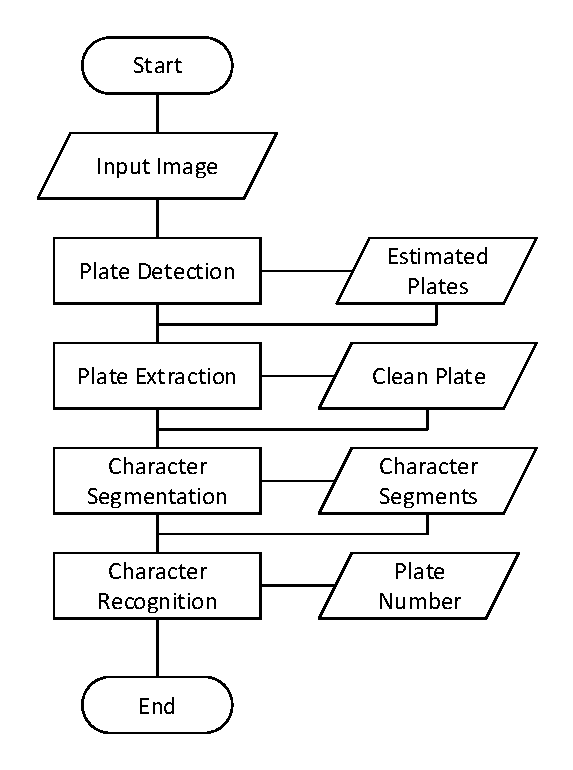
\includegraphics[width=0.8\linewidth]{./img/plots/overview}
	\caption{An overview of the plate detection procedure.} 
	\label{fig:ProcessOverview}
\end{figure}

\begin{description}
\item [Input Image] is a 24-bit colored image with red, green and blue channels.
\item [Preprocessing] stage applies several operations on input image to convert it into an image suitable for feature analysis for later stages. In our case, it also outputs general location of the plate.
\item [Plate Detection] analyses all plate like locations, and extract plates from them. Also it cleans the plate for segmentation.
\item [Segmentation] step is for splitting the characters from the plate. It is done so that the characters can be recognized by the OCR.
\item [Plate recognition] uses an OCR system to recognize individual characters and text images.
\end{description}

\end{document}






\section{Preprocessing}
This stage contains a sequence of steps that enhance the plate like regions of an image and output an image that can be used directly for the next stage - plate detection.

\subsection{Rescale}
By minimizing the size of an image we can reduce processing time dramatically. But reducing image may result in loss of information. From reviews, we decided to use the dimension: $640 \times 480$. We re-scale the input image into this dimension at first step. Figure \ref{fig:RescaledSample} shows a sample image.
\begin{figure} 
	\centering
	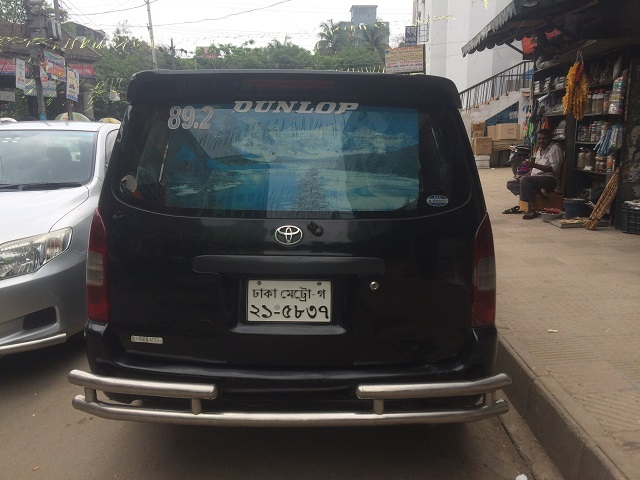
\includegraphics[width=.8\linewidth]{./img/sample/stage0.jpg}
	\caption{A sample input image (rescaled)}
	\label{fig:RescaledSample}
\end{figure}


\subsection{Gray Scale Conversion}
From the 24-bit color value of each pixels $(i, j)$ of the input image, we split the $R$, $G$, $B$ components . Then, 8-bit gray value is calculated using the following formula:
\begin{equation}
gray(i,j) = 0.59 * R(i,j) + 0.30 * G(i,j) + 0.11 * B(i, j)
\end{equation}
\begin{figure}
	\centering
	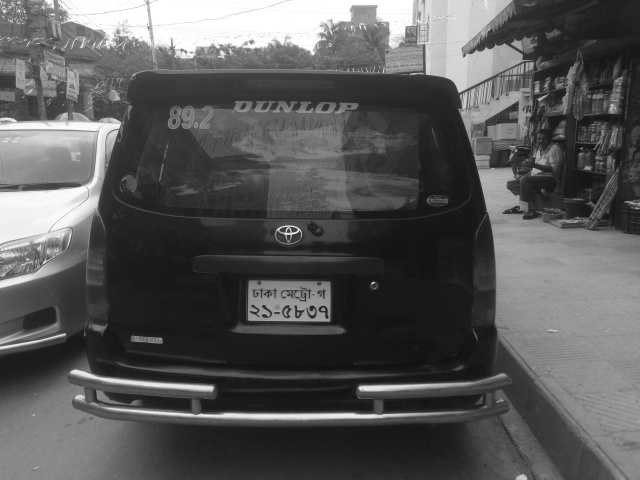
\includegraphics[width=.8\linewidth]{./img/sample/stage1.jpg}
	\caption{A sample gray-scale image} 
	 \label{fig:GraySample}
\end{figure}


\subsection{Vertical Edge Density}
The vertical {\it Sobel operator} (Equation \ref{eq:Sobel}) is used to calculated the edge density. 
\begin{equation} \label{eq:Sobel}
h =
  \begin{bmatrix}
    -1 & 0 & 1\\
    -2 & 0 & 2\\
    -1 & 0 & 1
  \end{bmatrix} 
\end{equation}

Which we could obtain by using $sobel$ function from OpenCV library:
\begin{lstlisting}[language=Python]
sobel = cv2.Sobel(img, cv2.CV_8UC1, 1, 0, ksize=3)
\end{lstlisting}

Next, we applied a low threshold value to the gradient image. In this case, we used an adaptive threshold technique called {\it Otsu’s Binarization} using an offset value of $85$, which we obtained empirically. Result is shown in Figure \ref{fig:SobelSample}
\begin{figure}
	\centering
	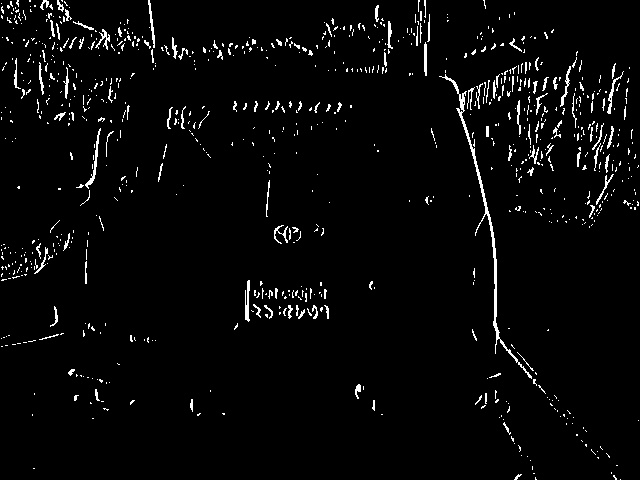
\includegraphics[width=.8\linewidth]{./img/sample/stage2.jpg}
	\caption{After applying Sobel Operator} 
	\label{fig:SobelSample}
\end{figure}

\subsection{Gaussian Filter}
In this step, 2D Gaussian filter is applied to the gradient image from previous step. We used a Gaussian kernel of size $60 \times 60$. To calculate the kernel the formula in Equation \ref{eq:GaussFilter} is used.
\begin{equation} \label{eq:GaussFilter}
g(i, j) = \dfrac{\alpha}{2\pi\sigma^2} \cdot e^{\frac{i^2 + j^2}{2\sigma^2}}
\end{equation}

Here, the blur coefficient $\alpha$ and the $\sigma$ are set empirically. We used $filter2D$ function to apply convolution of on the gradient image
\begin{lstlisting}[language=Python]
gauss = cv2.filter2D(sobel, cv2.CV_64F, kernel)
\end{lstlisting}

As a result we get a nicely blurred image (Figure \ref{fig:GaussianSample}).
\begin{figure} 
	\centering
	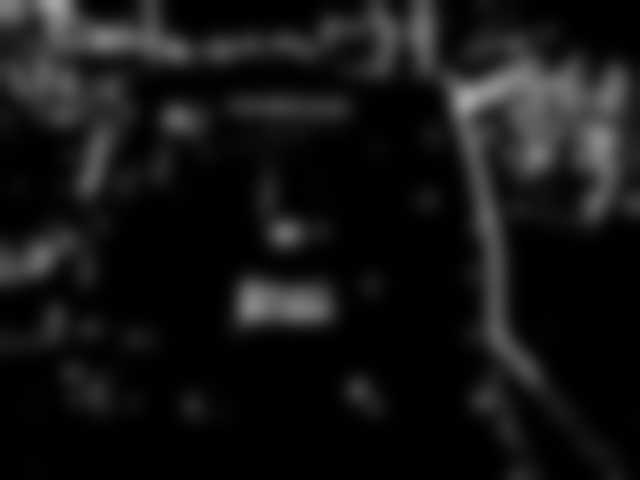
\includegraphics[width=.8\linewidth]{./img/sample/stage3.jpg}
	\caption{Applied the Gaussian Blur} 
	\label{fig:GaussianSample}
\end{figure}

\subsection{Image Enhancement}
We used the Gaussian image to increase the contrast of the image around plate like regions. The formula used is shown in Equation \ref{eq:Enhancement}.
\begin{equation} \label{eq:Enhancement}
I' = f(\rho W_g) (I - \bar{I}) + \bar{I}
\end{equation}
In the equation \ref{eq:Enhancement},\\
$\bar{I}$ = the mean intensity. \\
$I$ = the intensity of the original image. \\
$I'$ = the new enhanced image. \\
$W_g$ = normalized Gaussian image. \\ 
$\rho W$ = the standard deviation of Gaussian image, and \\
$f$ = the weighting function defined in Equation \ref{eq:WeightFunction}.

\begin{equation} \label{eq:WeightFunction}
f(\rho W_g) = 
\begin{cases} 
	\dfrac{3}{ \dfrac{2}{0.3^2} ( \rho W_g - 0.3)^2 + 1 },
    	& \mbox{if } 0 \leq \rho W_g < 0.3  
     \\
    
    \dfrac{3}{ \dfrac{2}{(0.5 - 0.3)^2} ( \rho W_g - 0.3)^2 + 1 },
    	& \mbox{if } 0.3 \leq \rho W_g < 0.5  
     \\
        
    1	& \mbox{if } \rho W_g \geq 0
\end{cases}
\end{equation} 

To increase the efficiency of the calculation the entire image is divided into $8 \times 8$ windows each having the size of $60 \times 80$. For each window we calculated weight and mean intensity using {\it Bilinear interpolation}. Also by using {\it numpy} library for matrix manipulation, we could dramatically decrease processing time.

Figure \ref{fig:EnhanceSample} shows the resultant image. The brightness of license plate area has significantly improved.
\begin{figure} 
	\centering
	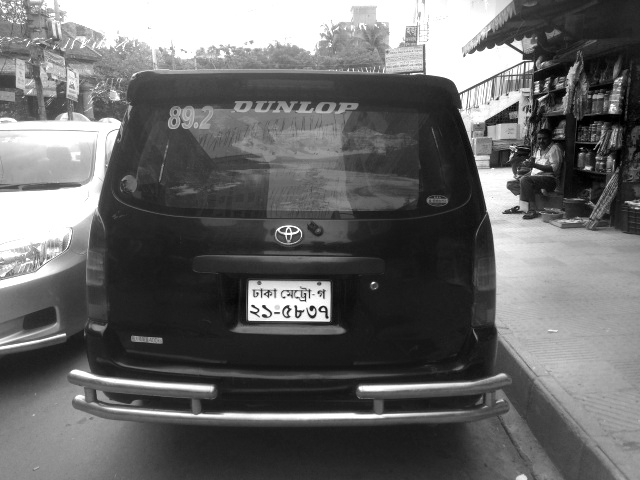
\includegraphics[width=.8\linewidth]{./img/sample/stage4.jpg}
	\caption{Enhanced Image} 
	\label{fig:EnhanceSample}
\end{figure}


\subsection{Matched Filter}
To detect the license plate, next step is to highlight plate like regions from the enhanced image. We used a mixture of Gaussian functions to emphasize the constancy of intensity values within plate-like regions along horizontal direction. Equation \ref{eq:MixtureModel} shows the mathematical model of this function. This function can properly model low edge densities above, below and at the middle of the car plate. 

\begin{equation} \label{eq:MixtureModel}
h(x, y) = 
\begin{cases} 
	A.exp \left(
    	\dfrac{ -\left(x - \dfrac{m}{6} \right)^2 }
        	{ 0.2 \sigma_x^2 } \right),                                      
    	& \mbox{for } 
        	0 \leq x \leq \dfrac{m}{3}, 
            0 \leq y \leq n     
    \\ \vspace{0.2cm}
    B.exp \left( 
    	\dfrac{ -\left(x - 
        			\left( \dfrac{m}{3} + \dfrac{m}{6} \right) 
                \right)^2 }
        	{ 2 \sigma_x^2 } \right),                
        & \mbox{for }
        	\dfrac{m}{3} \leq x \leq 2\dfrac{m}{6}, 
        	0 \leq y \leq n 
    \\ \vspace{0.2cm}
    A.exp \left( 
    	\dfrac{ -\left(x - 
        			\left( 2\dfrac{m}{3} + \dfrac{m}{6} \right) 
                \right)^2 }
        	{ 0.2 \sigma_x^2 } \right),
    	& \mbox{for } 
        	2\dfrac{m}{3} \leq x \leq m, 
            0 \leq y \leq n         
\end{cases}
\end{equation}


In the Equation \ref{eq:MixtureModel}, 
$A$ and $B$ are coefficients of the mixture model. These parameters are set empirically following the condition: $A > 0$ and $B < 0$. 
The symbol $\sigma_x$ is the variance of the main lobe toward x direction. 

This filtering process provides a strong response at plate-like regions (Figure \ref{fig:OriginalMixtureModel}). The result is compared against a predefined threshold value, which is around $80\%$ of the maximum intensity. We call this process as smoothing, and the threshold value as {\it smoothing cutoff}.

\begin{figure}
\begin{subfigure}{.5\textwidth}
  \centering
  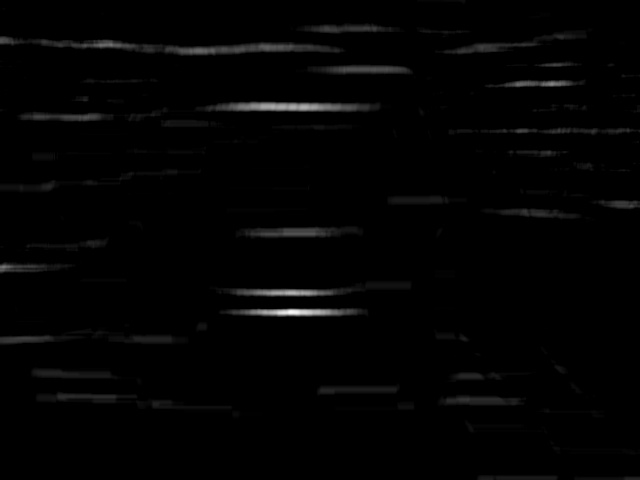
\includegraphics[width=.8\linewidth]{./img/sample/stage5-4.jpg}
  \caption{After applying the mixture model}
  \label{fig:OriginalMixtureModel}
\end{subfigure}
\begin{subfigure}{.5\textwidth}
  \centering
  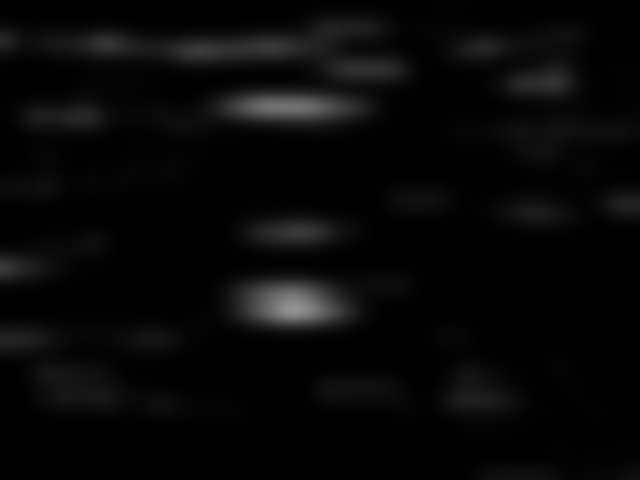
\includegraphics[width=.8\linewidth]{./img/sample/stage5-3.jpg}
  \caption{Gaussian blur on \ref{fig:OriginalMixtureModel}}
  \label{fig:BlurredMixtureModel}
\end{subfigure}
\begin{subfigure}{.5\textwidth}
  \centering
  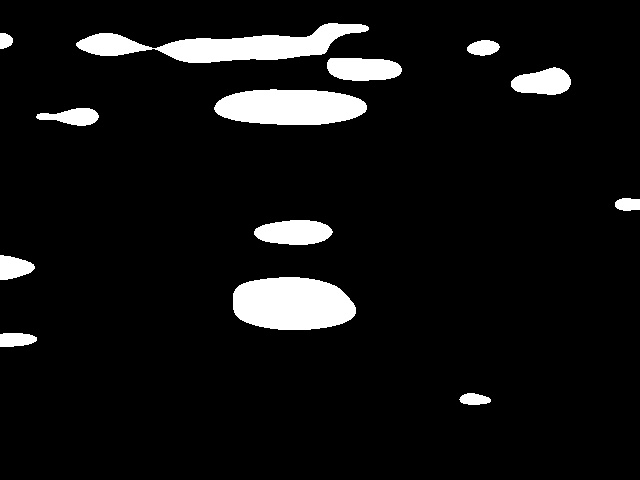
\includegraphics[width=.8\linewidth]{./img/sample/stage5-1.jpg}
  \caption{After applying adaptive threshold}
  \label{fig:ThresholdMixtureModel}
\end{subfigure}
\begin{subfigure}{.5\textwidth}
  \centering
  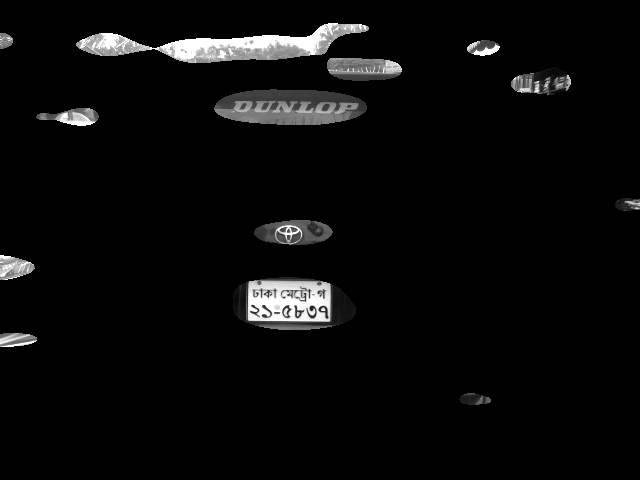
\includegraphics[width=.8\linewidth]{./img/sample/stage5-2.jpg}
  \caption{A see-through view of \ref{fig:ThresholdMixtureModel} with main image}
  \label{fig:GlassViewMixtureModel}
\end{subfigure}
\caption{Images after applying mixture model.}
\label{fig:MixtureModel}
\end{figure}


\subsection{Plate and regions extraction}
This step extracts the license plate and its bounding regions primarily. This does not detect actual license plate. But gives a close approximation to the location of the license plate. First we calculated all contours of the image calculated by mixture model. Next for each contours, we validated the bounding rectangle it is in. If the size of the bounding rectangle is valid, we extract the image of the area and region data. The extracted plates from the previous stage is shown in Figure \ref{fig:ExtractedPlates}.

\begin{figure}
\begin{subfigure}{.5\textwidth}
  \centering
  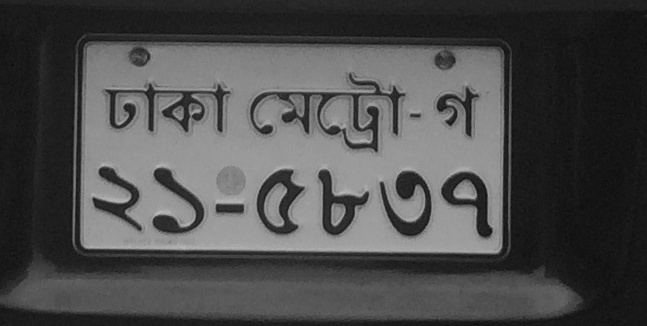
\includegraphics[width=.8\linewidth]{./img/sample/stage6-1.jpg}
  \caption{First estimation}
  \label{fig:FirstExtracted}
\end{subfigure}
\begin{subfigure}{.5\textwidth}
  \centering
  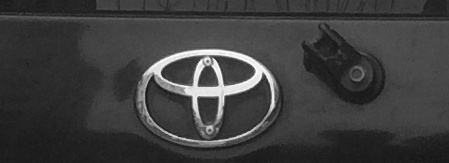
\includegraphics[width=.8\linewidth]{./img/sample/stage6-2.jpg}
  \caption{Second estimation}
  \label{fig:SecondExtracted}
\end{subfigure}
\begin{subfigure}{.5\textwidth}
  \centering
  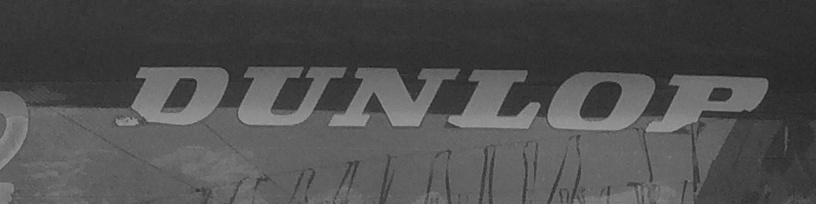
\includegraphics[width=.8\linewidth]{./img/sample/stage6-3.jpg}
  \caption{Third estimation}
  \label{fig:ThirdExtracted}
\end{subfigure}
\begin{subfigure}{.5\textwidth}
  \centering
  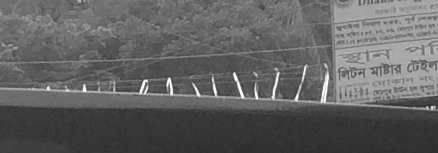
\includegraphics[width=.8\linewidth]{./img/sample/stage6-4.jpg}
  \caption{Fourth estimation}
  \label{fig:FourthExtracted}
\end{subfigure}
\caption{Estimated license plates.}
\label{fig:ExtractedPlates}
\end{figure}






\section{Plate Detection}
This section describes the procedure to localize the license plate using the outputs from preprocessing stage. 

\begin{figure} 
	\centering    
	{\it put an image here }
	\caption{An overview of the plate detection procedure.} 
	\label{fig:DetectionMethod}
\end{figure}

\subsection{Edge Analysis}
Before detectining edges we first applied a threshold value to the estimated license plates (Figure \ref{fig:ThresholdCanny}).
\begin{figure}
\begin{subfigure}{.5\textwidth}
  \centering
  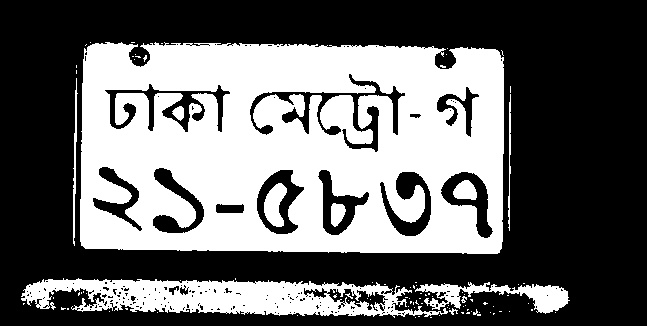
\includegraphics[width=.8\linewidth]{./img/sample/stage7-1.jpg}
\end{subfigure}
\begin{subfigure}{.5\textwidth}
  \centering
  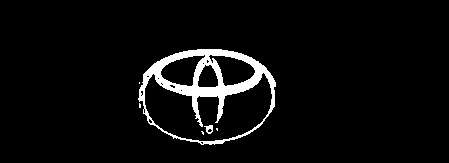
\includegraphics[width=.8\linewidth]{./img/sample/stage7-2.jpg}
\end{subfigure}
\begin{subfigure}{.5\textwidth}
  \centering
  
\includegraphics[width=.8\linewidth]{./img/sample/stage7-3.jpg}
\end{subfigure}
\begin{subfigure}{.5\textwidth}
  \centering
  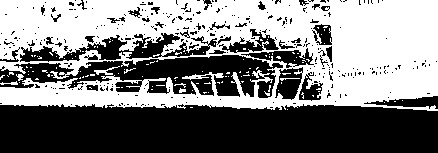
\includegraphics[width=.8\linewidth]{./img/sample/stage7-4.jpg}
\end{subfigure}
\caption{Applying threshold before Canny edge detection.}
\label{fig:ThresholdCanny}
\end{figure}

Canny Edge Detection is a popular edge detection algorithm. OpenCV has a direct function to it. We used the default function OpenCV provides to detect all edges of the localized estimated license plate image (Figure \ref{fig:CannyEdges}). 
\begin{lstlisting}[language=Python]
canny = cv2.Canny(img, 100, 200, L2gradient=True)
\end{lstlisting}

\begin{figure}
\begin{subfigure}{.5\textwidth}
  \centering
  
\includegraphics[width=.8\linewidth]{./img/sample/stage8-1.jpg}
  \caption{Edges of \ref{fig:FirstExtracted}}
\end{subfigure}
\begin{subfigure}{.5\textwidth}
  \centering
  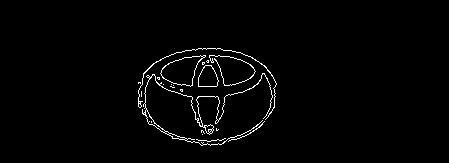
\includegraphics[width=.8\linewidth]{./img/sample/stage8-2.jpg}
  \caption{Edges of \ref{fig:FirstExtracted}}
\end{subfigure}
\begin{subfigure}{.5\textwidth}
  \centering
  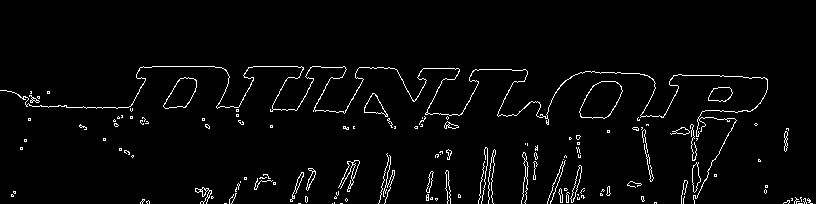
\includegraphics[width=.8\linewidth]{./img/sample/stage8-3.jpg}
  \caption{Edges of \ref{fig:FirstExtracted}}
\end{subfigure}
\begin{subfigure}{.5\textwidth}
  \centering
  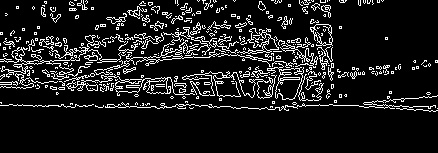
\includegraphics[width=.8\linewidth]{./img/sample/stage8-4.jpg}
  \caption{Edges of \ref{fig:FirstExtracted}}
\end{subfigure}
\caption{Result of Canny edge detecton algorithm.}
\label{fig:CannyEdges}
\end{figure}



\subsection{Contour Analysis}
Canny edge detection works perfectly for most cases and provides an easy to detect contours around plate borders. After passing the canny image to the OpenCV's $findContours$ function, we get a set of contours. For each of these contours several parameters are checked before selecting a contours as a possible plate.

In this steps, some of the estimated candidate from previous stages fall out. In Figure \ref{fig:ContourImage}, all detected the contours are highlighted.
\begin{figure}
    \centering
    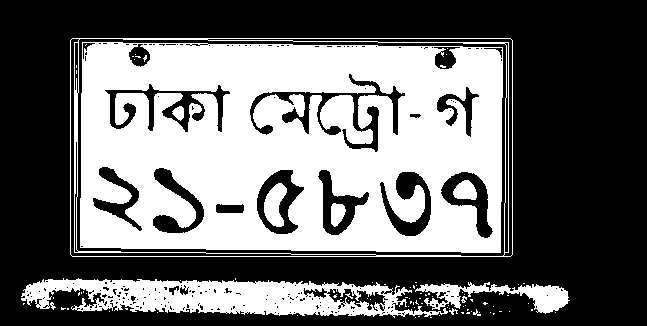
\includegraphics[width=.7\linewidth]{./img/sample/stage9.jpg}
    \caption{Only remaining candidate after contour analysis}
    \label{fig:ContourImage}
\end{figure}

\subsubsection{Width and Height}
The width and height of the detected contour should be above a minimum margin to be recognizable by the OCR. We set the minimum width = $30$ pixels and minimum height = $75$ pixels for estimated plate.

\subsubsection{Area Ratio}
Next we check if the area of the contour is greater than the $10\%$ of the entire image. Remember, we got this image by localizing the plate like regions in pre-processing stage. A possible plate should not have the area below $10\%$ of the entire image.
\begin{equation}
area\_ratio = \dfrac{contour\_area}{image\_area }
\end{equation}

\subsubsection{Aspect Ratio}
Equation \ref{eq:AspectRatio} shows the calculation of aspect ratio of the contour image. From review and observations, we set the minimum value of aspect ratio to $0.3$ and maximum to $0.6$.
\begin{equation} \label{eq:AspectRatio}
aspect\_ratio = \dfrac{contour\_height}{contour\_width}
\end{equation}

\subsubsection{Rotation}
The rotation can be found by the $minAreaRect$ function from OpenCV. 
\begin{lstlisting}[language=Python]
angle = cv2.minAreaRect(cnt)[0]
\end{lstlisting}
If $10 \leq |angle| \leq 80$ we skipped the contour. Because otherwise the contour will be too much skewed to be recognized by any OCR.

\subsection{Extraction}
The region information we get from the previous step is used here to extract the plate image from the original image. We also rotate the image to match with the rotation angle found in previous step. This rotation is done by calculating a rotation matrix of scale $1$ using a OpenCV function:
\begin{lstlisting}[language=Python]
# Calculating rotation matrix M
M = cv2.getRotationMatrix2D(\
		     (center_y, center_x), rotation, 1.0)
\end{lstlisting}

The variable $rotation$ here is calculated from the $minAreaRect$'s $angle$ using Equation \ref{eq:ExtractionAngle}.
\begin{equation} \label{eq:ExtractionAngle}
rotation = 
\begin{cases} 
	-angle, & \mbox{if } angle \leq 45\\
    90 - angle, & \mbox{if } angle > 45
\end{cases}
\end{equation}

For convenience, the extracted plate image is rescaled into a dimension of $500 \times 250$. Figure \ref{fig:FinalPlate} shows a sample.
\begin{figure}
    \centering
    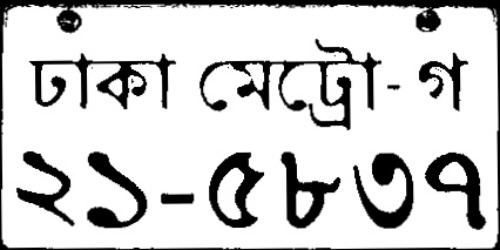
\includegraphics[width=.7\linewidth]{./img/sample/stage10.jpg}
    \caption{The extracted plate after rotation and scaling}
    \label{fig:FinalPlate}
\end{figure}


\subsection{Converting to Black and White}
The image from previous stage is need to be converted in Black and White for convenience. But Bangladeshi license plate has two types of plates. White text on black plate for private cars and black text on white plate for public ones. To be accurate we first converted the image into black and white using two filters: $THRESH_BINARY$ one time and $THRESH_BINARY_INV$ the other. Then compared the ratio of non-zero pixels of each image. The image which has lesser mean most probably is the black and white image. 
\begin{lstlisting}[language=Python]
    # normal binary threshold
    bnw1 = cv2.threshold(np.uint8(img), cfg.BNW_THRESH, 255,
                         cv2.THRESH_BINARY | cv2.THRESH_OTSU)[1]

    # inverse binary threshold
    bnw2 = cv2.threshold(np.uint8(img), cfg.BNW_THRESH, 255,
                         cv2.THRESH_BINARY_INV | cv2.THRESH_OTSU)[1]

    # calculate ratio of non-zero pixels
    row, col = img.shape
    area = row * col
    ratio1 = cv2.countNonZero(bnw1) / area
    ratio2 = cv2.countNonZero(bnw2) / area

    # return image with lower ratio
    bnw = bnw2
    if ratio1 < ratio2:
        bnw = bnw1
    # end if
    bnw[bnw <= 127] = 0
    bnw[bnw > 127] = 255
    return bnw
\end{lstlisting}

Figure \ref{fig:BlackAndWhite} shows the conversion between black and white images using the above algorithm for different types of license plates.

\begin{figure}
\begin{subfigure}{.5\textwidth}
  \centering
  
\includegraphics[width=.8\linewidth]{./img/sample/bnw-1.jpg}
  \caption{A private license plate}
  \label{fig:PrivatePlate}
\end{subfigure}
\begin{subfigure}{.5\textwidth}
  \centering
  
\includegraphics[width=.8\linewidth]{./img/sample/bnw-2.jpg}
  \caption{Black and white image of \ref{fig:PrivatePlate}}
\end{subfigure}
\begin{subfigure}{.5\textwidth}
  \centering
  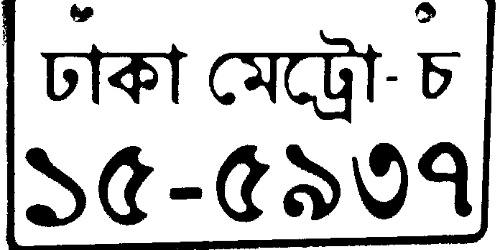
\includegraphics[width=.8\linewidth]{./img/sample/bnw-3.jpg}
  \caption{A public license plate}
  \label{fig:PublicPlate}
\end{subfigure}
\begin{subfigure}{.5\textwidth}
  \centering
  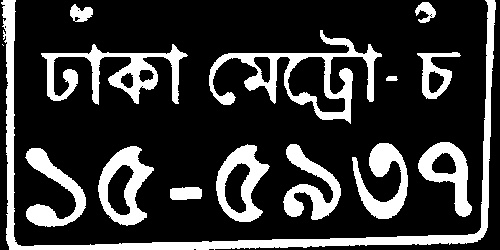
\includegraphics[width=.8\linewidth]{./img/sample/bnw-4.jpg}
  \caption{Black and white image of \ref{fig:PublicPlate}}
\end{subfigure}
\caption{Black and white conversion of two types of image}
\label{fig:BlackAndWhite}
\end{figure}

\subsection{Border removal}
Removing the borders of an image is tough job due to the diversity of plates and their origins. In our methods, we first removed the top, bottom, left and right border using OpenCV's $floodFill$ function. We checked all the pixels of first $20$ rows and applied flood-fill on any non-black pixels. Similarly we check bottom $5$ rows, from left first $12$ columns and from right the first $12$ columns.

\subsection{More De-noising}
Only removing border is not enough to completely clear the plate image. We used contour analysis to blackout the remaining dots in the image that could not possibly be a letter. 

Figure \ref{fig:CleaningStage} shows the result of border and noise removal.
\begin{figure}
\begin{subfigure}{.5\textwidth}
  \centering
  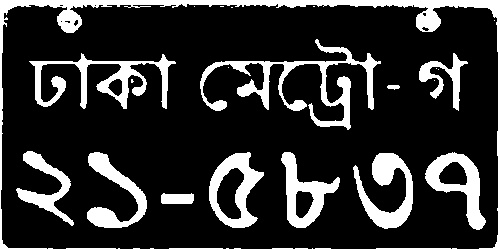
\includegraphics[width=.8\linewidth]{./img/sample/stage11.jpg}
  \caption{Noisy image}
\end{subfigure}
\begin{subfigure}{.5\textwidth}
  \centering
  
\includegraphics[width=.8\linewidth]{./img/sample/stage12.jpg}
  \caption{Clean image}
\end{subfigure}
\begin{subfigure}{0.9\textwidth}
  \centering
  
\includegraphics[width=.8\linewidth]{./img/sample/stage13.jpg}
  \caption{Clean image}
\end{subfigure}
\caption{After applying Border removal and De-noising}
\label{fig:CleaningStage}
\end{figure}


\section{Segmentation}
\subsection{Horizontal Segmentation}
\subsection{Vertical Segmentation}

\section{Alternative Procedure}
\subsection{Find plate in part of the frame (ROI)}
\subsection{Find the plate using previous locations}

\section{Plate Recognition}
\subsection{Translate coordinates}
\subsection{Extract original plate}
\subsection{Cleaning image}
\subsection{Converting to Binary image}

\section{Character segmentation}
\subsection{Horizontal projection}
\subsection{Vertical projection}


\end{document}